\documentclass[a4paper,12pt]{article}
\usepackage[pdftex]{graphicx}
\usepackage[font=scriptsize,labelfont=bf,labelsep=endash]{caption}
\usepackage[font=scriptsize,labelfont=bf]{subfig}
\usepackage{setspace}
\usepackage{wrapfig}
\usepackage{fullpage}
\usepackage{sidecap}

\title{Automated Image Classification for Vespidae Family of Wasps}

\author{
	Adrian Teng-Amnuay\\
	Taiwan Forest Research Institute: Taipei, TW\\
	University of California, San Diego\\
	atengamn@ucsd.edu
}

\date{September 1, 2011}

\doublespacing
\begin{document}
\maketitle

\begin{singlespace}
\begin{abstract}
	Taxonomic identification has traditionally been carried out by individuals with years of experience and in-depth knowledge of the particular taxa. The process of identifying specimens can often be time-consuming and tedious. We present a system for automated image classification on a small subset of the Vespidae family of wasps. While our system still has much room for improvement, we hope to demonstrate that automated systems are becoming increasingly prevalent and provide a feasible alternative to human-driven identification methods.
\end{abstract}
\end{singlespace}

\section{Introduction}
The Vespidae family of wasps consists of several thousand species. To the untrained eye, some species may be more difficult to distinguish than others (Figure~\ref{fig:comparisons}). In light of the ambiguity of certain species and the repetitive nature of manually identifying specimens, automated systems become an attractive option. In this paper, we establish a workflow for automated image classification and discuss the advantages and disadvantages of our system. 

\begin{figure}[t]
	\centering
	\subfloat[Easy to distinguish]{
		\label{fig:easy}
		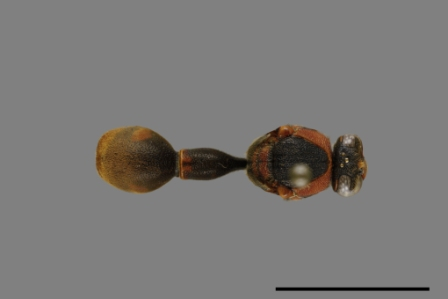
\includegraphics[width=0.25\textwidth]{compare/Eumenes}
		\includegraphics[width=0.25\textwidth]{compare/Delta}
	}
	\subfloat[Difficult to distinguish]{
		\label{fig:difficult}
		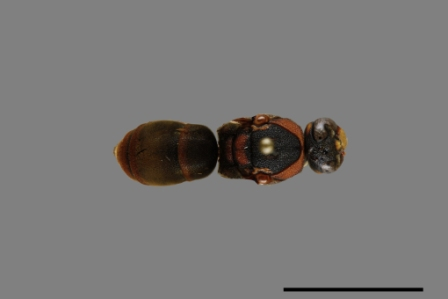
\includegraphics[width=0.25\textwidth]{compare/Anterhynchium}
		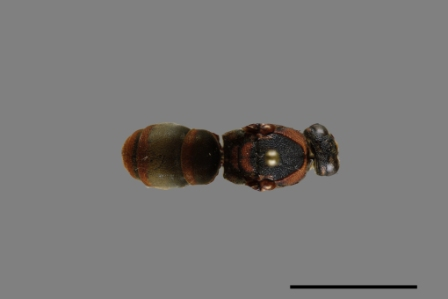
\includegraphics[width=0.25\textwidth]{compare/Orancistrocerus}
	}
	\caption{}
	\label{fig:comparisons}
\end{figure}

\section{Related Work}
Considerable research has already been done on automated identification of insects. Oregon State University and University of Washington have made remarkable progress with their project on automatic stonefly identification~\cite{stonefly:article}, while reliable approaches have been demonstrated in bee identification using only images of wings or bee faces~\cite{automated_taxon:book}. 

Most forms of image analysis share common challenges due to the amount of information that is lost from projecting a three-dimensional object onto a two-dimensional image. Some of the main challenges that persist in object recognition are variation in pose or lighting, and scene segmentation. Depending on the severity of these conditions, reliable recognition may not even be possible. Dealing with these issues is still an active field of research in Computer Vision, so it is important to take these factors into consideration when capturing images and designing the system.

\section{System Implementation}
In the following sections, we discuss the image classification pipeline in detail. We make extensive use of the OpenCV Library~\cite{opencv_library} for its flexible matrix data structures, its robust algorithms geared towards feature extraction and image processing, and for its wide selection of machine learning models.

\subsection{Scoping the Problem}
In this section, we discuss the need to simplify different aspects of the problem. Our main goal is not to develop a state-of-the-art system, but to establish a foundation for automated image classification, where future work can easily be continued and thorough documentation is readily available.

\begin{figure}[t]
	\centering
	\subfloat{
		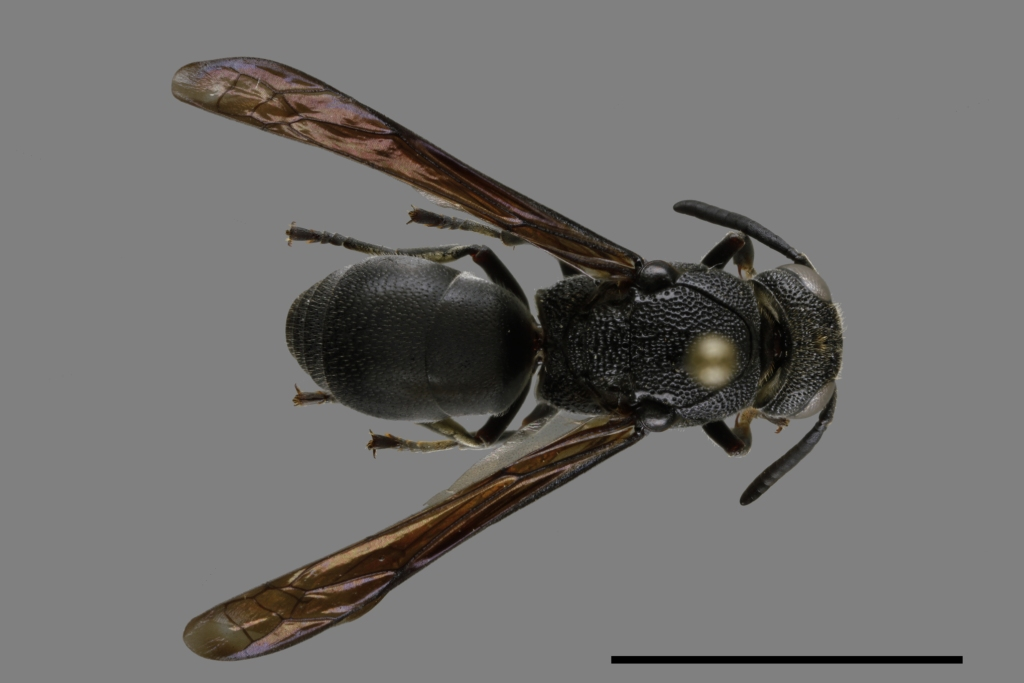
\includegraphics[width=0.125\textwidth]{working16/1}
		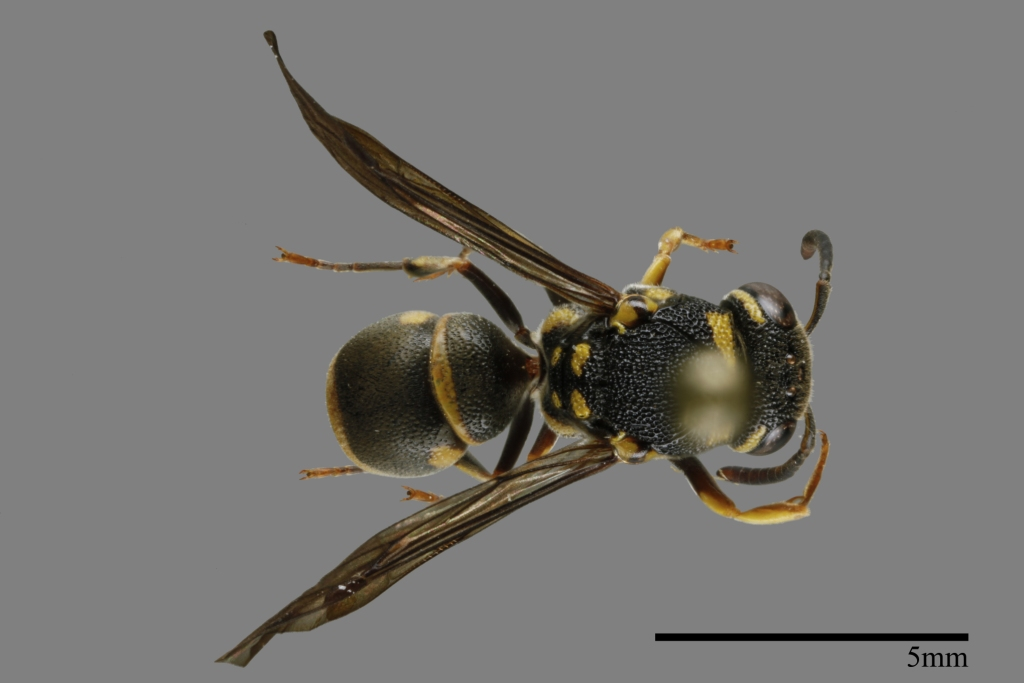
\includegraphics[width=0.125\textwidth]{working16/2}
		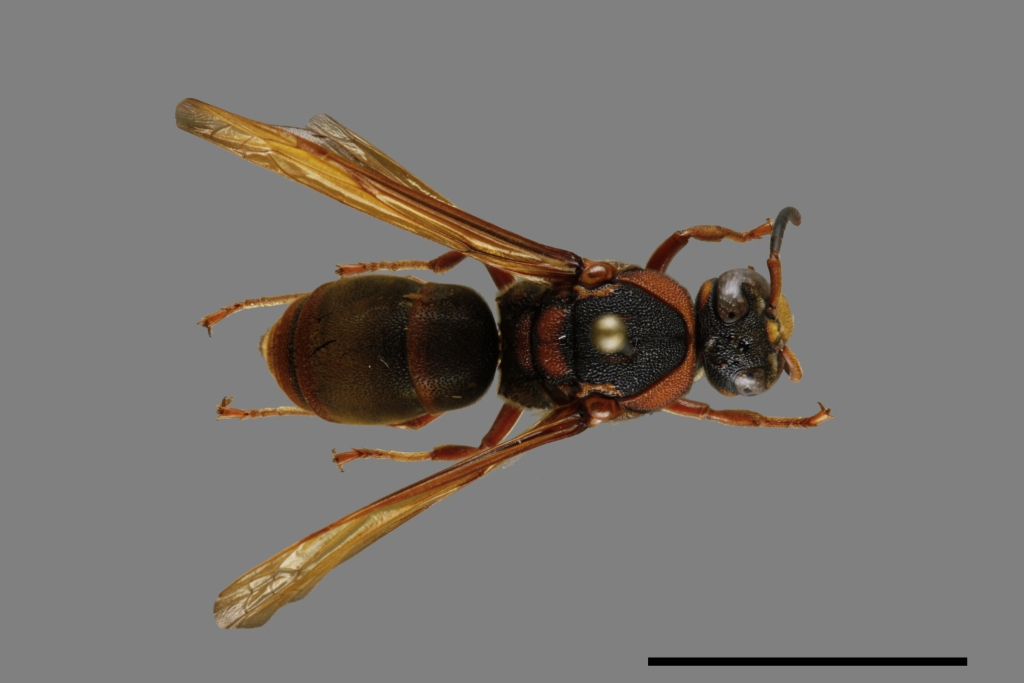
\includegraphics[width=0.125\textwidth]{working16/3}
		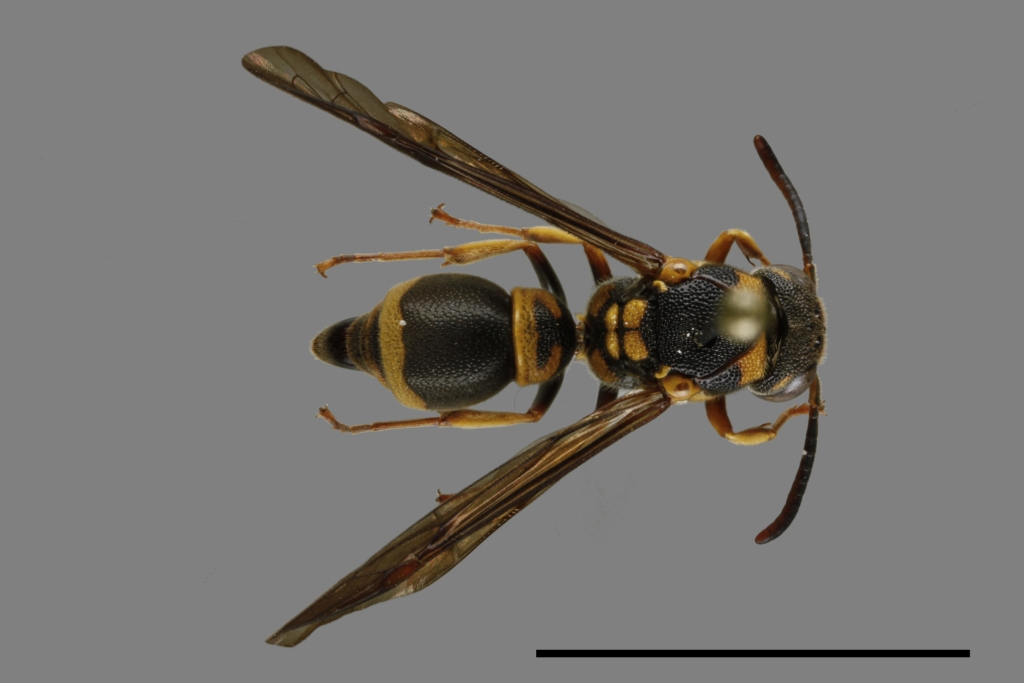
\includegraphics[width=0.125\textwidth]{working16/4}
		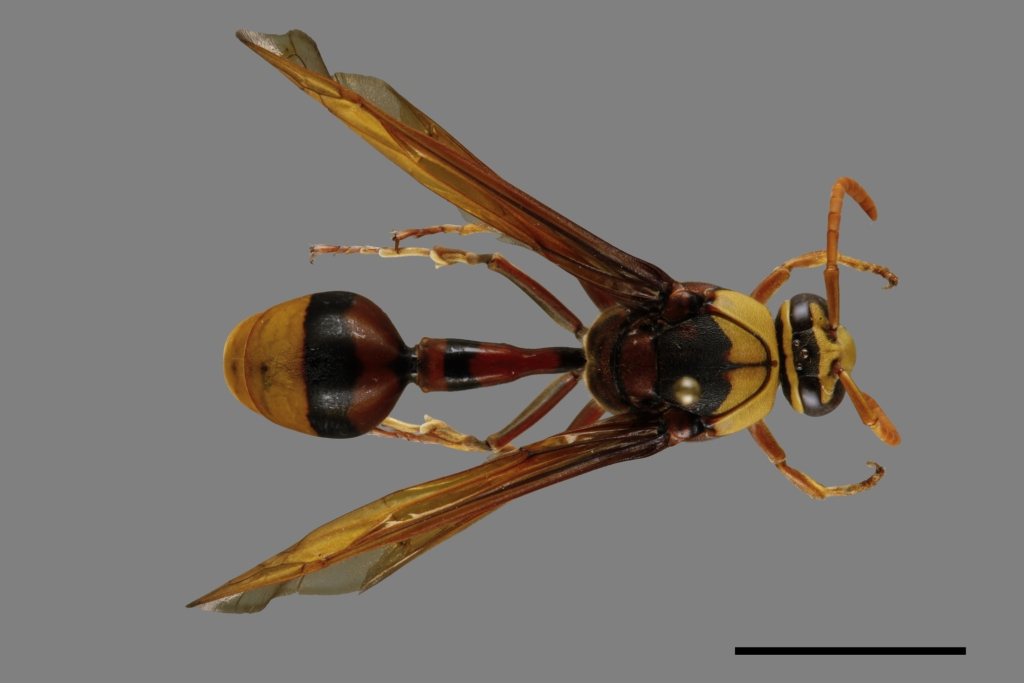
\includegraphics[width=0.125\textwidth]{working16/5}
		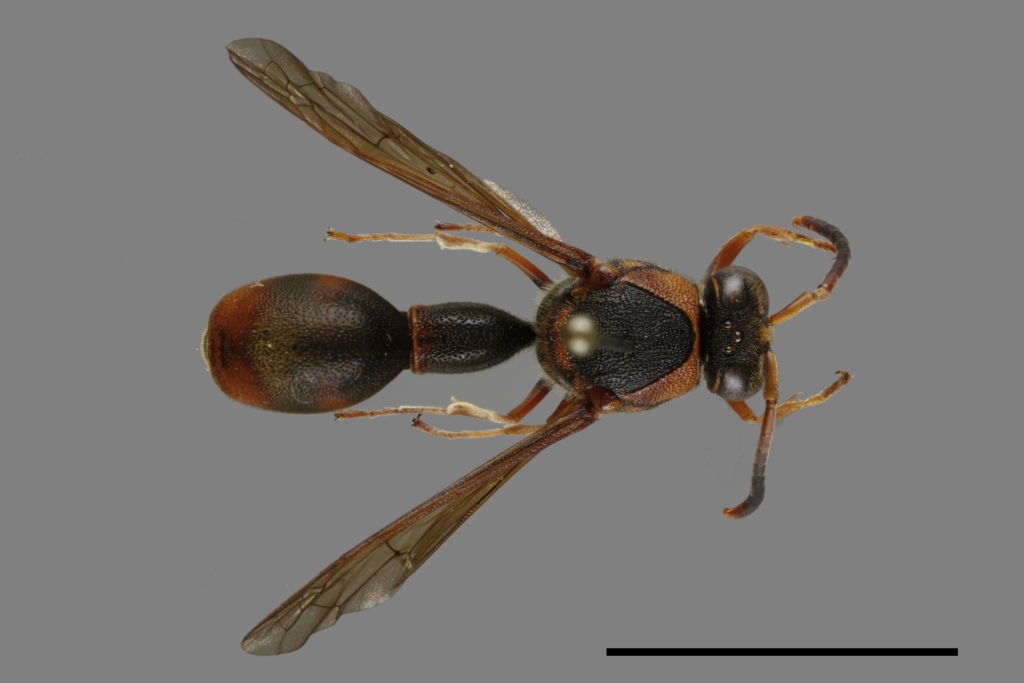
\includegraphics[width=0.125\textwidth]{working16/6}
		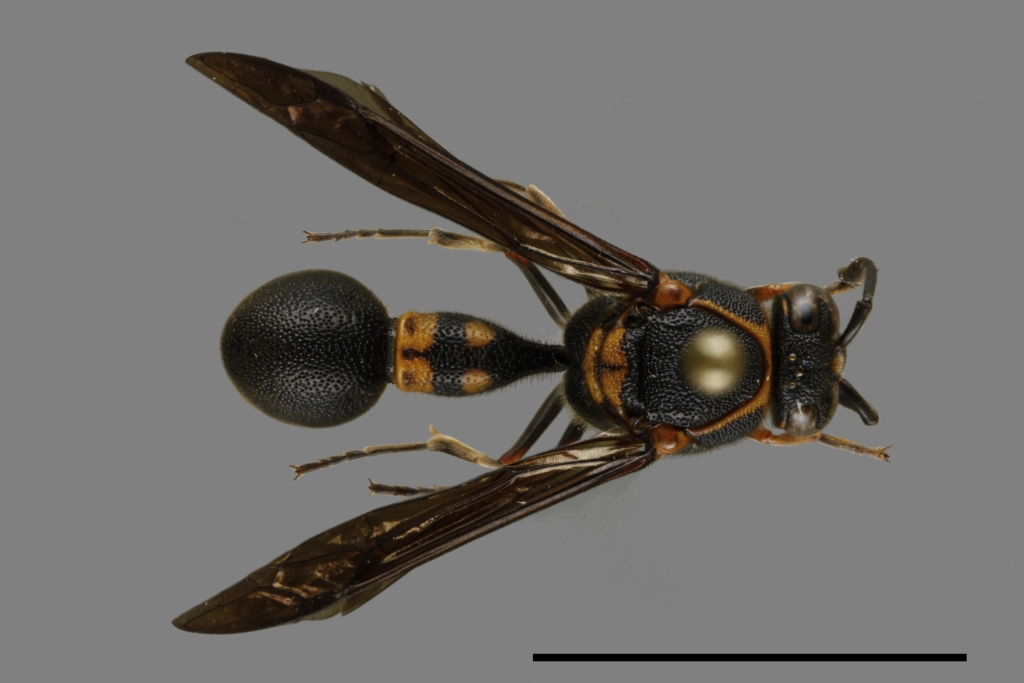
\includegraphics[width=0.125\textwidth]{working16/7}
		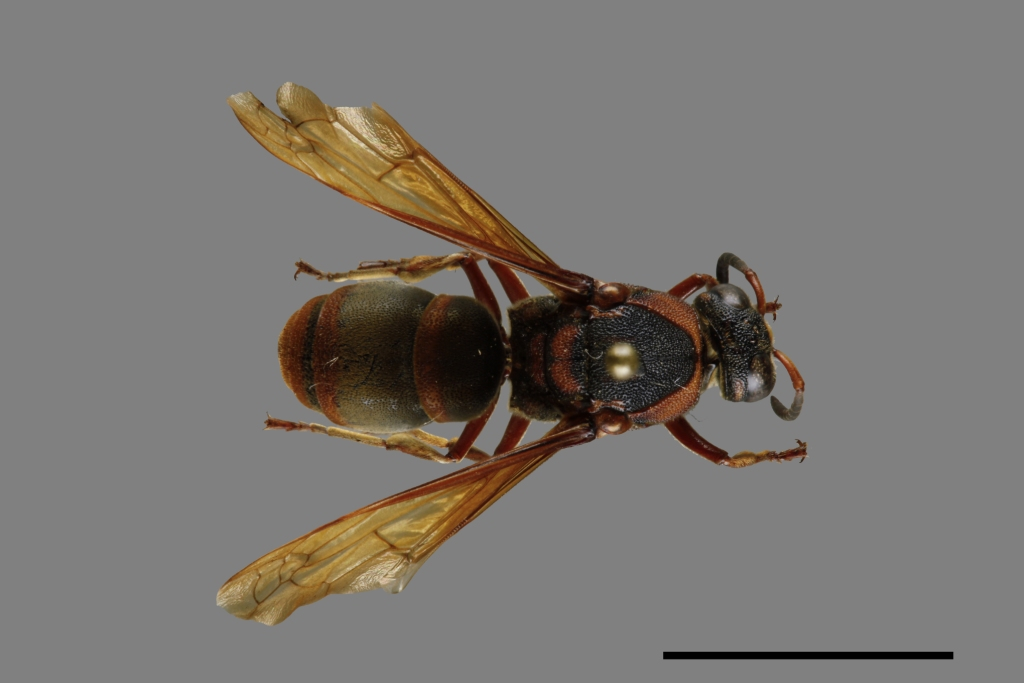
\includegraphics[width=0.125\textwidth]{working16/8}
	}
	\\
	\subfloat{
		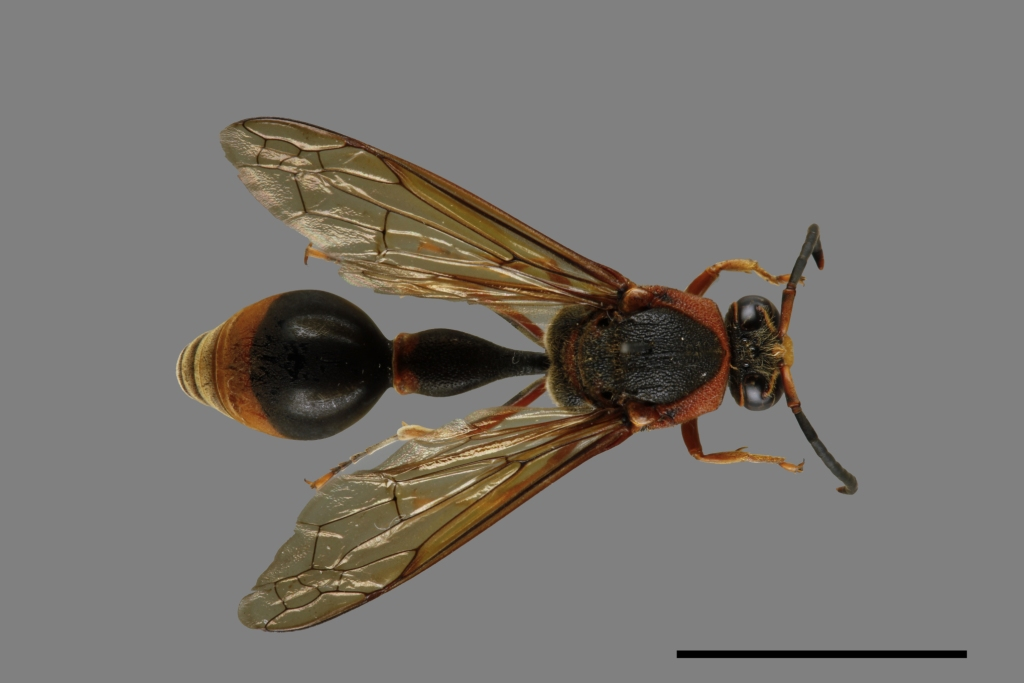
\includegraphics[width=0.125\textwidth]{working16/9}
		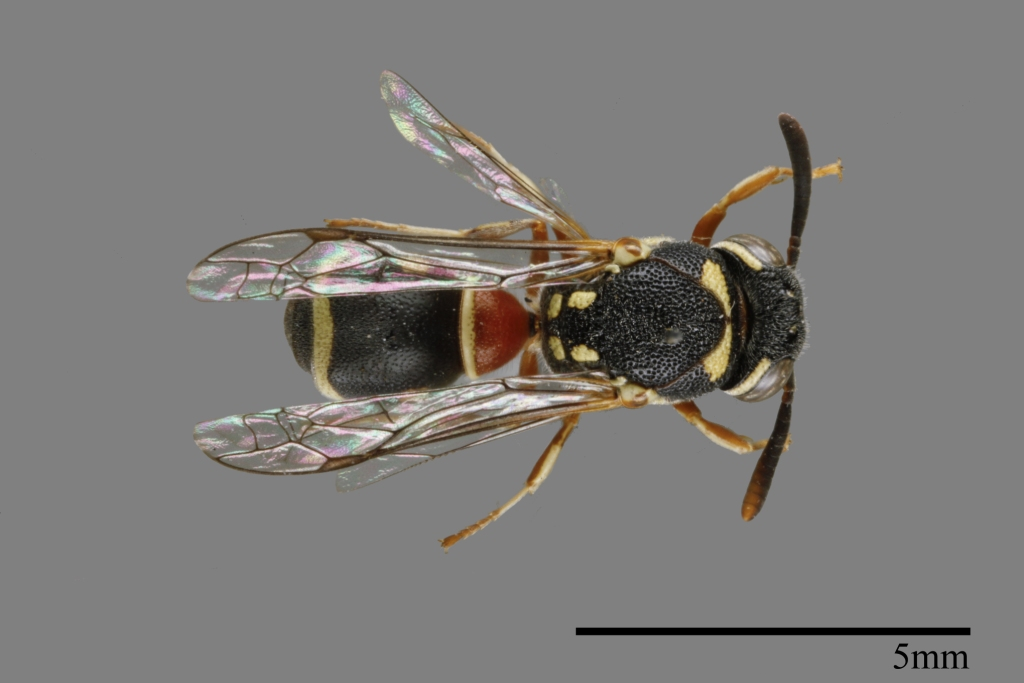
\includegraphics[width=0.125\textwidth]{working16/10}
		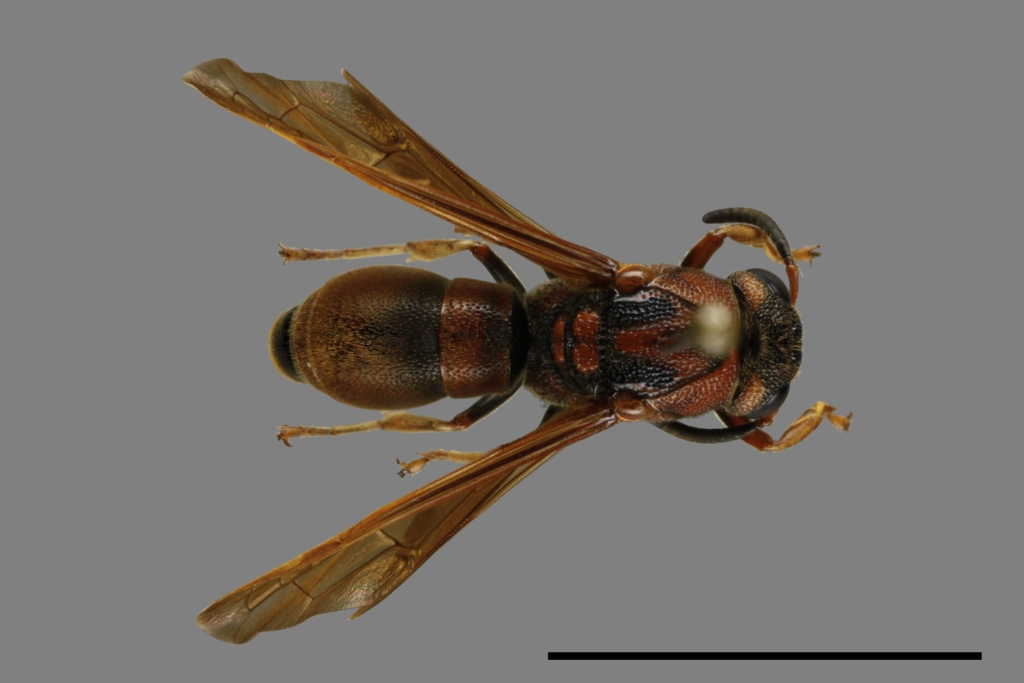
\includegraphics[width=0.125\textwidth]{working16/11}
		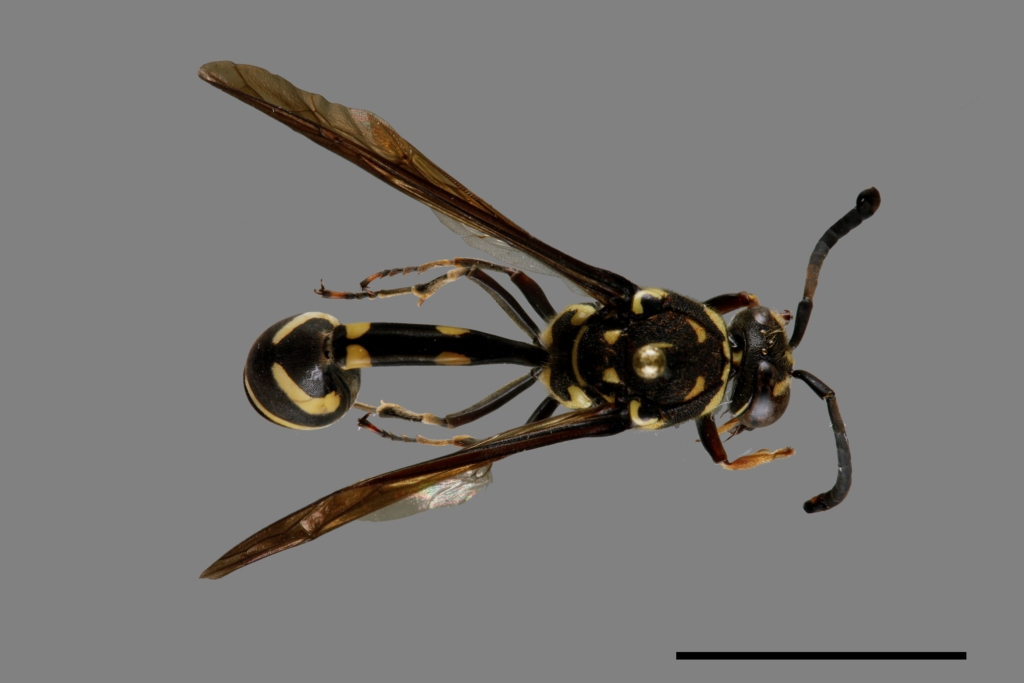
\includegraphics[width=0.125\textwidth]{working16/12}
		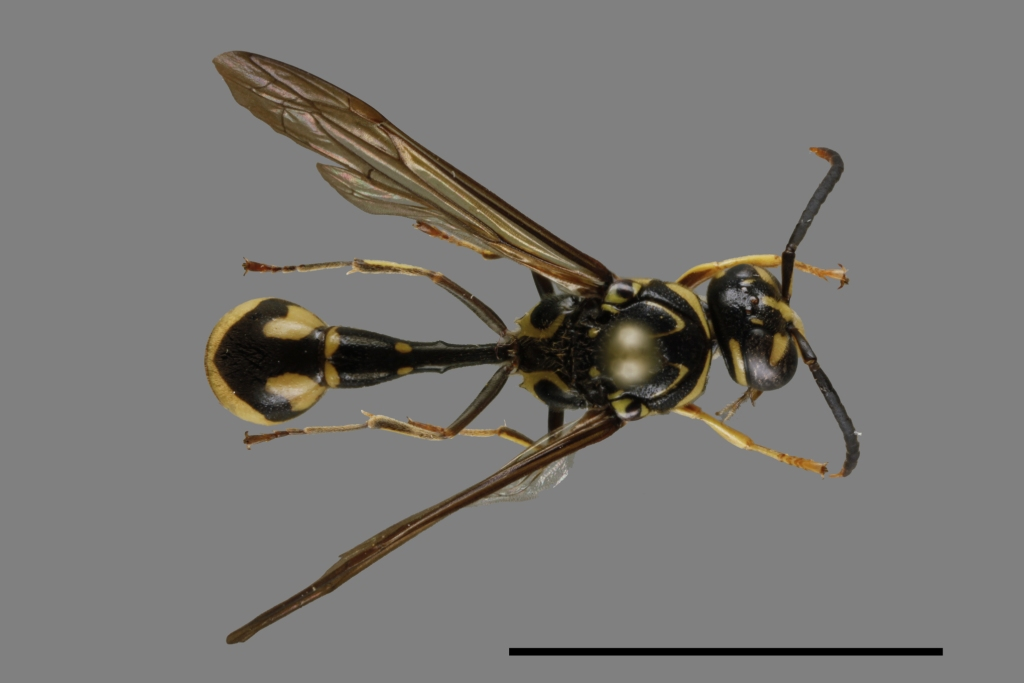
\includegraphics[width=0.125\textwidth]{working16/13}
		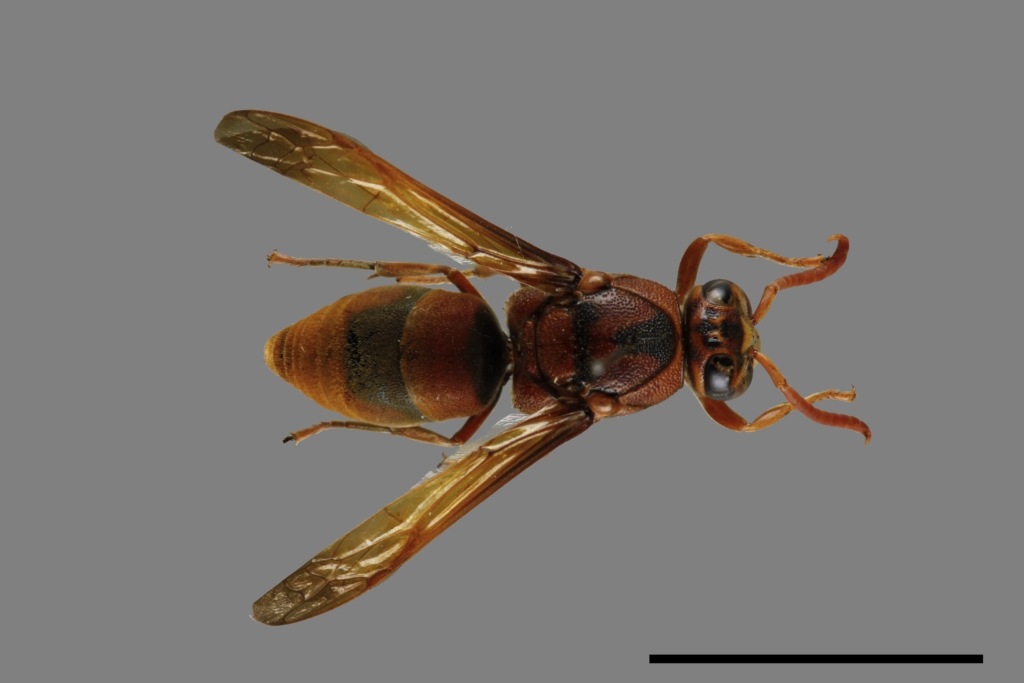
\includegraphics[width=0.125\textwidth]{working16/14}
		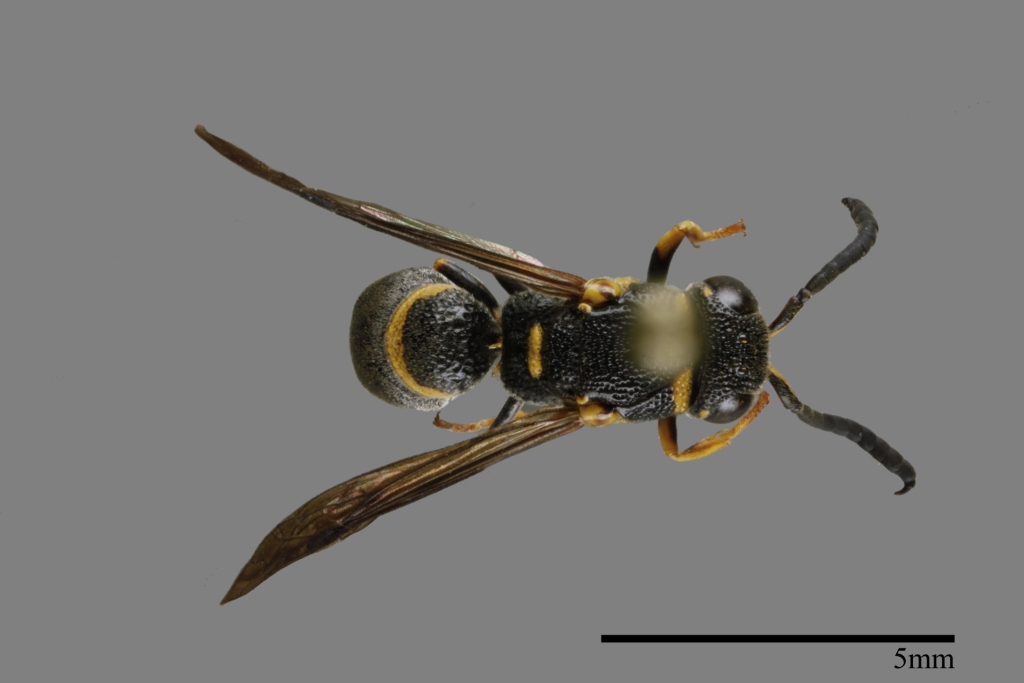
\includegraphics[width=0.125\textwidth]{working16/15}
		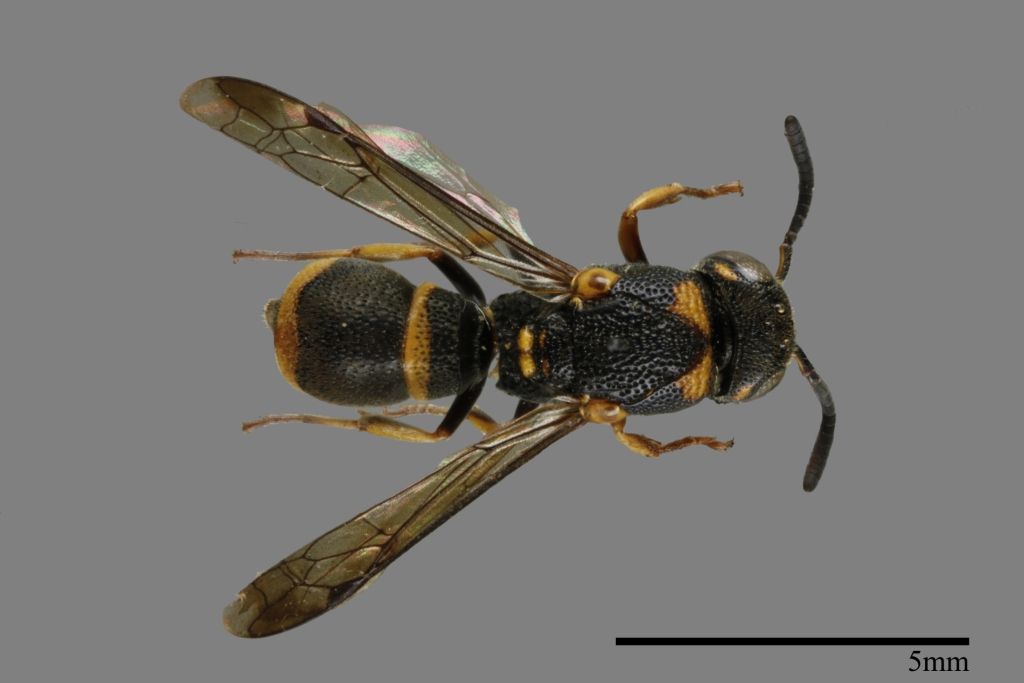
\includegraphics[width=0.125\textwidth]{working16/16}
	}
	\caption{Row one: Allorhynchium argentatum, Antepipona biguttata, Anterhynchium flavomarginatum formosicola, Apodynerus f.formosensis, Delta pyriforme, Eumenes l.labiatus, Eumenes tosawae, Orancistrocerus drewseni. Row two: Oreumenes decoratus, Paraleptomenes m. miniatus, Pararrhynchium ornatum suuteri, Phimenes flavopictus formosanus, Pseumenesd depressus, Rhynchium quinquecinctum brunneum, Stenodynerus chinesis, Subancistrocerus kankauensis.}
	\label{fig:working-set}
\end{figure}

\begin{wrapfigure}[9]{r}{0.25\textwidth}
	\vspace{-30pt}

	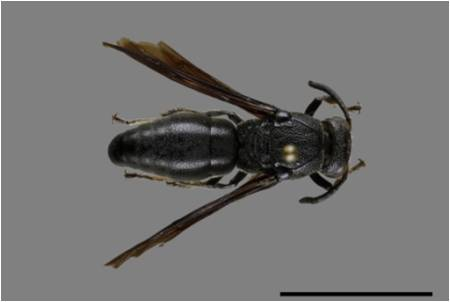
\includegraphics[width=0.25\textwidth]{nowings/wings}
	\\\\
	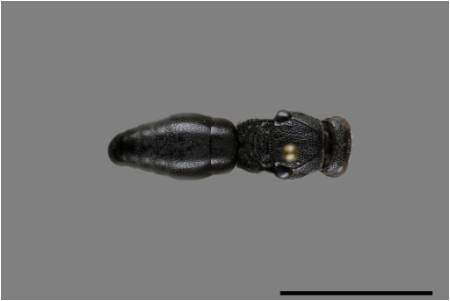
\includegraphics[width=0.25\textwidth]{nowings/nowings}
	
	\caption{Example before and after manual wing segmentation}
	\label{fig:wing_seg}
\end{wrapfigure}

Our system is based on statistical learning approaches, which means that there needs to be a significant number of examples for each species for the model to learn from. Having too few samples leads to overfitting, meaning that the model cannot generalize. Out of the 35 species in the Taiwan Forest Research Institute (TFRI) database, we choose to work with 16 of them (Figure~\ref{fig:working-set}) because the rest only contain a few samples each. 

Another issue that our system does not account for is variation in wing pose and inconsistency in wing color/lighting caused by the transparency of the wing. Segmenting the wings out is a difficult problem, and so we opt to manually segment the wings using a picture editor instead as in Figure~\ref{fig:wing_seg}.

\subsection{Image Preprocessing}
Image preprocessing is essentially filtering out noise from the data and preserving most of the important information. The first step is to down-sample the images in order to compress and blur them. Compression helps to  remove redundant data and speed up computation, while blurring helps to smoothen out the edges as well as get rid of background noise. After the down-sampling, an algorithm determines which blob represents the wasp body and crops the image as detailed in Figure~\ref{fig:preprocessing}.

\begin{figure}[t]
	\centering
	\subfloat[Blur image]{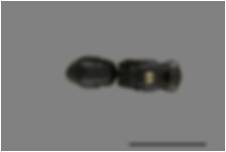
\includegraphics[width=0.23\textwidth]{cropROI/1}} \hfill
	\subfloat[Create binary image by thresholding pixels]{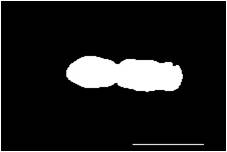
\includegraphics[width=0.23\textwidth]{cropROI/2}} \hfill
	\subfloat[Fit rectangle around largest blob]{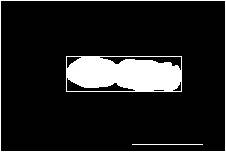
\includegraphics[width=0.23\textwidth]{cropROI/3}} \hfill
	\subfloat[Crop image using bounding rectangle]{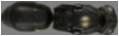
\includegraphics[width=0.23\textwidth]{cropROI/4}\label{fig:black-sample}}
	\caption{}
	\label{fig:preprocessing}
\end{figure}

\subsection{Feature Extraction}
Choosing features is perhaps the most creative step in the pipeline. Features can be anything that describe the object such as number of legs, weight, height, color, etc., but the difficulty lies primarily in extracting the features. Whether the features are useful or not for classification is easily determined from the machine learning models.

At a high level, the two main features we use for Vespidae classification are color and shape. There are many different ways to describe these features at a low level, so we discuss our approach in detail.

\subsubsection{Color Histograms}
For describing color, we extract 2-D Hue and Saturation (H-S) histograms as in Figure~\ref{fig:HS-histogram}. We believe that the HSV space captures color more realistically than does the standard RGB space. We also disregard the ``Value'' channel to provide some invariance to lighting. From our experiments, 30 hue bins and 32 saturation bins worked best though it was not tested thoroughly. We also found that computing color histograms from multiple regions of the image provided more information than a single global histogram from the entire image. 
\begin{wrapfigure}[8]{r}{0.5\textwidth}
	\vspace{-10pt}
	\centering
	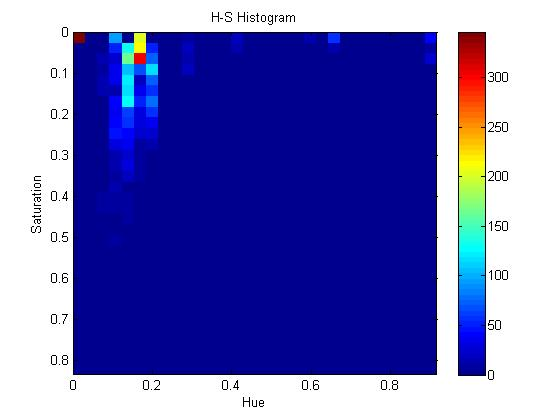
\includegraphics[width=0.5\textwidth]{hs/hs-ex}
	\caption{H-S Histogram extracted from sample in Figure~\ref{fig:black-sample}}
	\label{fig:HS-histogram}
\end{wrapfigure}
This is clearly attributed to the fact that colors are not randomly distributed about the body for each specimen, they are characterized by patterns on each species. Furthermore allowing these regions to overlap as in Figure~\ref{fig:overlap-color} showed increased performance. We found that seven windows, each half-overlapped, worked best from our experiments.
\begin{SCfigure}[50][h]
	\vspace{-10pt}
	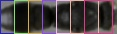
\includegraphics[width=.25\textwidth]{hs/wind}
	\caption{Seven overlapped windows for calculating color histograms}
	\label{fig:overlap-color}
\end{SCfigure}

\subsubsection{Histogram of Oriented Gradients}
For encoding shape information, we use Histogram of Oriented Gradients (HOG) as detailed in~\cite{hog:article}. The idea of overlapping windows for color histograms in the previous section was actually inspired by HOG features. HOG features (see Figure~\ref{fig:hog-example} for example) are a robust shape descriptor that are illumination invariant, but not size or orientation invariant.
 \begin{wrapfigure}[6]{r}{.25\textwidth}
	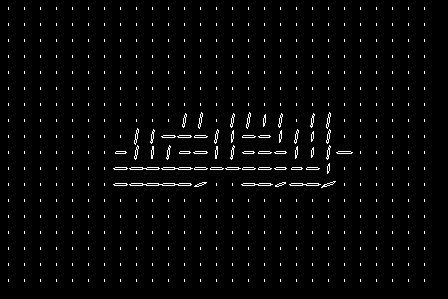
\includegraphics[width=.25\textwidth]{hs/hog}
	\caption{HOG feature representation of a specimen}
	\label{fig:hog-example}
\end{wrapfigure}
It is necessary to normalize the cropped image sizes before extracting the HOG features, so we simply choose the average dimensions of 34x117 pixels for this normalization. For the HOG parameters we use an 8x8 cell size, 3x3 block size, and seven unsigned bins. We did not test extensively, but these parameters worked best out of several sets of parameters that were tested during our experiments.

\subsubsection{Feature Reduction}
The last step of feature extraction is to reduce the number of features, while still retaining the most important ones. High feature dimensionality, also referred to as the ``curse of dimensionality,'' is problematic because computational overhead grows exponentially with the number features. Using 30 hue bins and 32 saturation bins produces a feature length of 960, and overlapping seven of these totals to 6720 features. Using the specified parameters and image sizes for the HOG descriptor produces 3780 features. 

We turn to Principal Component Analysis (PCA) to project the feature vectors onto a lower dimensional space, while capturing most of the variance in the data. From our experiments there was no significant loss in performance after reducing the number of color features to 300 and HOG features to 200.

\subsection{Model Selection}
Out of the statistical models we experimented with such as k-Nearest Neighbor and Decision Trees, Multiclass Support Vector Machines (SVM) performed the best. One-against-one SVMs outperformed one-against-rest SVMs, but due to limited time we choose to work with one-against-rest SVMs for convenience.

\subsubsection{Probabilistic Output}
Rather than have our model simply output the class label for a given specimen, it is useful to convert the output to a set of probabilistic outputs or confidence values. For example, given an unknown specimen $x$, our model should be able to produce probabilities $P(class_{i} \mid color(x))$ and $P(class_{i} \mid shape(x))$, where $0 \le i < \left|classes\right|$ and $classes$ is the alphabetically ordered set of species in Figure~\ref{fig:working-set}.

Under the assumption that color and shape are independent, we can now combine the probabilities using a rule of statistical inference known as conditional independence. We obtain the joint probability as follows,
\begin{equation}
P(class_{i} \mid color(x)~\verb#and#~shape(x)) = P(class_{i} \mid color(x)) * P(class_{i} \mid shape(x))
\label{eq:probs}
\end{equation}

\section{Results}
We validate our model using 10 fold cross-validation, while ensuring that each validation set contains roughly the same distribution of species for each fold. To assess the performance of our model, we introduce confusion matrices. 

Confusion matrices are a visual representation for how often the model confuses one class for another. A value located at row $m$, column $n$, represents the number of times an instance of class $m$ was predicted as class $n$. Consequently, numbers along the diagonal of the matrix represent correctly classified instances, while numbers everywhere else in the matrix represent misclassified instances.

Figures~\ref{fig:conf-color}~and~\ref{fig:conf-hog} show the confusion matrices for Multiclass SVM trained on color features and shape features, respectively, along with the total number of images per class and individual class accuracies. The indices of the matrix correspond to the alphabetically ordered set of species in Figure~\ref{fig:working-set}.

\begin{figure}[h]
	\subfloat[Color features]{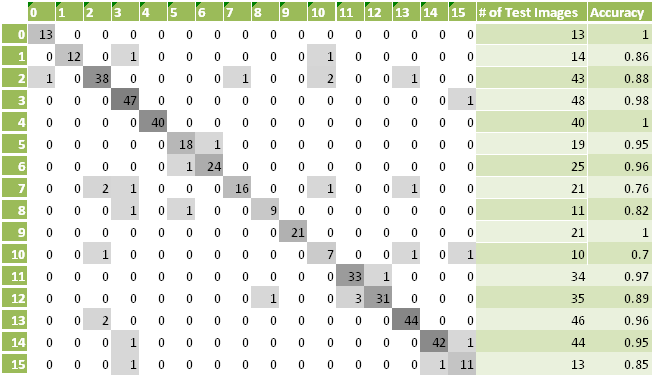
\includegraphics[width=0.48\textwidth]{confmat/color}\label{fig:conf-color}}
	\hfill
	\subfloat[Shape features]{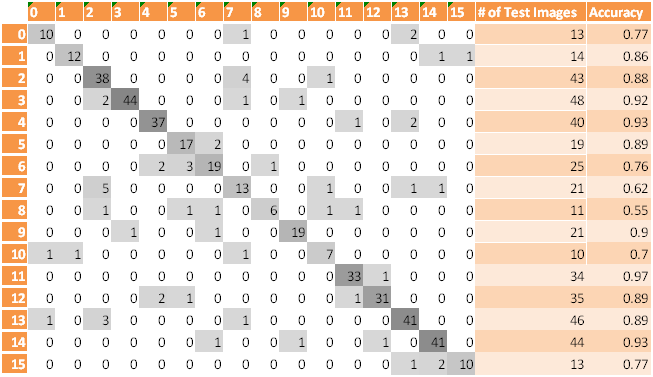
\includegraphics[width=0.48\textwidth]{confmat/hog}\label{fig:conf-hog}}
	\caption{Confusion Matrices for models trained on color and shape features independently}
\end{figure}

The overall accuracy of the model using only color features is 406 out of 437 samples correctly identified, or $92.906 \pm 4.534 \%$ ($\pm$ the standard deviation across the ten folds). The overall accuracy of the model using only shape features is 378 out of 437 samples correctly identified, or $86.499 \pm 4.843 \%$.

Finally, using equation~\ref{eq:probs} we can produce a model that takes both color and shape into account when classifying specimens. Figure~\ref{fig:conf-both} shows the confusion matrix for this new model. The overall accuracy using both color and shape features is 420 out of 437 samples correctly identified, or $96.110 \pm 1.810 \%$.

\begin{figure}[t]
	\centering
	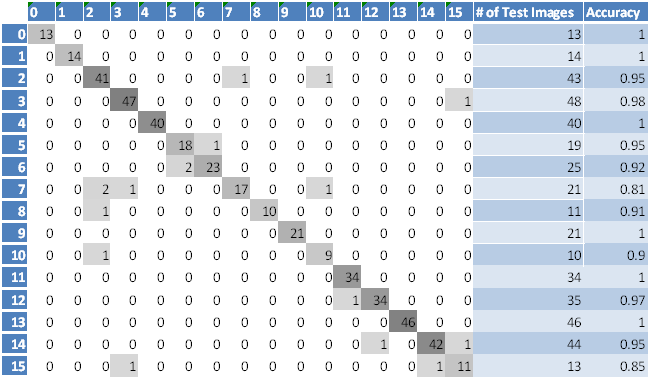
\includegraphics[width=0.6\textwidth]{confmat/both}
	\caption{Confusion Matrix for model combining color and shape features}
	\label{fig:conf-both}
\end{figure}

\section{Discussion and Conclusion}
We have developed a novel prototype for automatic classification of wasps, achieving an overall accuracy of about 96\%. However, there are still several unaddressed issues with our system that we discuss in more detail in the following section.

Combining cues for color and shape shows significant improvement over using either of them individually. In addition, the standard deviation across the folds decreased, implying that the new model was less dependent on the training data. We hope that our progress has demonstrated the potential for automated classification systems, and we also hope that our work will inspire more research dedicated to automated taxon identification.

\section{Future Work}
We now discuss the limitations of our system, and offer suggestions for dealing with them.

\subsection{Wing Segmentation}
Currently, the system only handles the manually edited photos of wasps without wings. The variation in wingspreads is problematic because it not only changes the underlying shape of the wasp, it also introduces a wide spectrum of different colors.

Our suggestion for dealing with this problem is to basically determine a rectangular region of interest that fits over the wasp body, similarly to the preprocessing step shown in Figure~\ref{fig:black-sample}. This region can be estimated via some form of template matching on the wasp bodies. Some key features to use for the template matching might be HOG features or the bilateral axis of symmetry in conjunction with other image moment features.

\subsection{Tuning Parameters}
Throughout this paper we discussed several parameters that were chosen as a result of our experiments such as cropped image dimensions, number of color histogram bins, and HOG parameters. The SVM parameters and probabilistic output function were not mentioned, but they were also determined in a similar fashion.

The preceding parameters are likely to be non-optimal as they were chosen manually based on our intuition. An optimization problem can be defined in terms of constraints on the parameters and a goal to maximize some objective value on performance. Solving this optimization problem would yield an optimal set of arguments, but whether or not it can be solved efficiently is a different issue.

\footenote{Acknowledgements}
The PRIME program is funded by the National Science Foundation (OISE-0710726) with additional support from Calit2 and PRAGMA. First and foremost, I want to the mentors at TFRI, Dr. Chau Chin Lin, Dr. Sheng-Shan Lu, and Dr. Yu-Hwang Wang, for hosting the project and supervising my stay in Taiwan. I'd also like to thank my mentor Dr. Tony Fountain at Calit2 for his insight and expertise on the Machine Learning aspect of the project, and Professor Serge Belongie at UCSD for his feedback and advice on the Computer Vision aspect. And finally, I want to thank Principal Investigator on the NSF award for PRIME, Dr. Gabriele Wienhausen, Principal Investigator (PI) of PRAGMA and co-PI of the PRIME NSF award, Dr. Peter Arzberger, the program manager of both PRIME and PRAGMA, Teri Simas, Director of Opportunities Abroad and Faculty-Led Programs at the UCSD Programs Abroad Office, Jim Galvin, and Assistant Director of the Academic Internship Program at UCSD, Tricia Taylor-Oliveira.


\bibliographystyle{unsrt}
\bibliography{PRIMEPaper2011}

\end{document}